\documentclass[11pt]{article}
\usepackage[margin=1.0in]{geometry}
\usepackage{ragged2e}
\usepackage{amsmath}    % Expanded math operations for papers
\usepackage{amssymb}
%\usepackage{esvect}    % Vector notation for mathematics
\usepackage{graphicx}
\usepackage{wrapfig}    % Format figures more appropriately
\usepackage{hyperref}   % Enable hyperlink support
\usepackage{fancyhdr}   % Allow headers and footers customized
\usepackage{titlesec}   % Allow customization of section headers
\usepackage{wrapfig}    % So I can wrap figures around my text
\usepackage{enumitem}	% Align things in the itemize environment
%\usepackage{subcaption}
\usepackage{subfig}
\usepackage[font=small,skip=0pt]{caption}

% Set up code environment
\usepackage{listings}
\usepackage{color}

\definecolor{mygreen}{RGB}{28,172,0} % color values Red, Green, Blue
\definecolor{mylilas}{RGB}{170,55,241}

\lstset{language=Matlab,%
    %basicstyle=\color{red},
    breaklines=true,%
    morekeywords={matlab2tikz},
    keywordstyle=\color{blue},%
    morekeywords=[2]{1}, keywordstyle=[2]{\color{black}},
    identifierstyle=\color{black},%
    stringstyle=\color{mylilas},
    commentstyle=\color{mygreen},%
    showstringspaces=false,%without this there will be a symbol in the places where there is a space
    numbers=left,%
    numberstyle={\tiny \color{black}},% size of the numbers
    numbersep=9pt, % this defines how far the numbers are from the text
    emph=[1]{for,end,break},emphstyle=[1]\color{red}, %some words to emphasise
    %emph=[2]{word1,word2}, emphstyle=[2]{style},    
}

% Set graphics path
\graphicspath{ {Figures/} }

% Reformat section headers
\titleformat{\section}{\normalfont\large\bfseries}{\thesection}{1em}{}[{\titlerule[0.8pt]}]
\titleformat{\subsection}{\normalfont\large\bfseries}{\thesubsection}{1em}{}
\titleformat{\subsubsection}{\normalfont\normalsize\bfseries}{\thesubsubsection}{1em}{}

% Define page header and footer
\pagestyle{fancy}
\fancyhf{}
\lhead{Seaborn • Buchanan • Sambolu}
\rhead{April 30, 2019}
\lfoot{ECE 460}
\rfoot{Page \thepage}

% Define paragraph spacing
\newcommand{\parSpace}{\vspace{0.5cm}}


\begin{document}



%
%%---------------------------------------------------------------------------------------------------| PROJECT APPROACH
%

\begin{Large}\begin{center}
DTMF Digit Detection Algorithm
\end{center}\end{Large}


%
%%---------------------------------------------------------------------------------------------------| PROJECT APPROACH
%

\section{Project Approach}

This project is almost identical to the technical challenges we faced in ECE 301, discrete time signals and systems. The challenge, as discussed in person with Dr. Lu, was to adapt our code from ECE 301 to improve upon our existing Dual Tone Multiple Frequency (DTMF) Detection model. In particular, Dr. Lu took issue with our approach of manually segmenting our input signals, therefore effectively eliminating the noise and timing challenges imposed by the problem statement. Our solution to this issue was to create a moving window DTMF detection system which replied upon an ecosystem of functions to quickly and generally solve smaller technical challenges.


%
%%---------------------------------------------------------------------------------------------------| PROCESS
%

\section{Moving Window Process}

Within our function ecosystem, we identified three tasks which needed to be accomplished: finding frequency peaks, identifying key pressed from peaks and managing a moving window system to manage detection and to avoid duplicate true positives.


\subsection{TwinPeaks.m}
\label{TwinPeaks}

\vspace{-0.1cm}
\textbf{function fPair = TwinPeaks( sample, freq )}
\vspace{0.3cm}

The twin peaks function is the heart of the DTMF detection operation. It performs a short fast-Fourier transform on the current window and forms an amplitude spectrum. This spectrum will illustrate noise below 600 Hz and will also show the peaks of the dual-tone frequencies between 600 Hz and 2000 Hz if they are present. Instead of applying a high pass filter with a cutoff of 600 Hz, thus eliminating noise, our algorithm saves valuable computing time by only analyzing the frequency range which interests us: 600 to 2000 Hz.

\parSpace

Using the spectrum, we find the two greatest peaks in our DTMF range and return them as a vector. By creating this function we can generalize our approach so that it can analyze any window width for any sampling rate of any recording.


\subsection{IdentifyKey.m}

\vspace{-0.1cm}
\textbf{function [match, kVal] = IdentifyKey( freqPair, tol )}
\vspace{0.3cm}

The next function used in our software was a system to take peak frequencies and check them against a table of DTMF pairs. We designed this function with a tolerance input which can be calibrated accordingly. If the input frequency pairs were within $\pm$ tol of a valid frequency pair then the function returned $\text{match} = \text{True}$ as well as the $\text{kVal}$ variable which stored the key pressed. If no valid pair was detected then it returned $\text{match} = \text{False}$. The match variable enabled process flow control outside of our lower-level functions.


\subsection{DTMF.m}
\label{DTMF}

\vspace{-0.1cm}
\textbf{function phone\_number = DTMF ( sample, time, frequency, window\_width, ext, plt )}
\vspace{-0.1cm}

Combining the efforts of its sub-functions, the DTMF function manages the logic of the algorithm. In particular, the moving window approach demands the detection of digits and the avoidance of duplicates when the window steps to the next section. Our system bypasses this issue by relying on the above functions instead of having all of the code under one MATLAB file. This enabled us to easily repeat functions and develop a higher level logic.

\parSpace

The window begins looking at the first \textit{window\_width} number of values in the sample and automatically assigns a step size of half the \textit{window\_width}, ensuring that no digits can be missed due to the window overlap. The window steps through the sample and waits until it receives a \textit{match} from \textit{IdentifyKey.m}, see Figure ~\ref{WindowStages} part A. At that point, it appends the matched key to the \textit{phone\_number} variable and steps through subsequent sample windows to avoid duplicates, Figure ~\ref{WindowStages} part B. When it samples a window without valid dual tone frequencies, it exits the loop and iterates through the sample until it collides into another key press, Figure ~\ref{WindowStages} part C. At this point it repeats the process until it runs out of data to sample.

\begin{figure}[h!]
	\begin{center}
		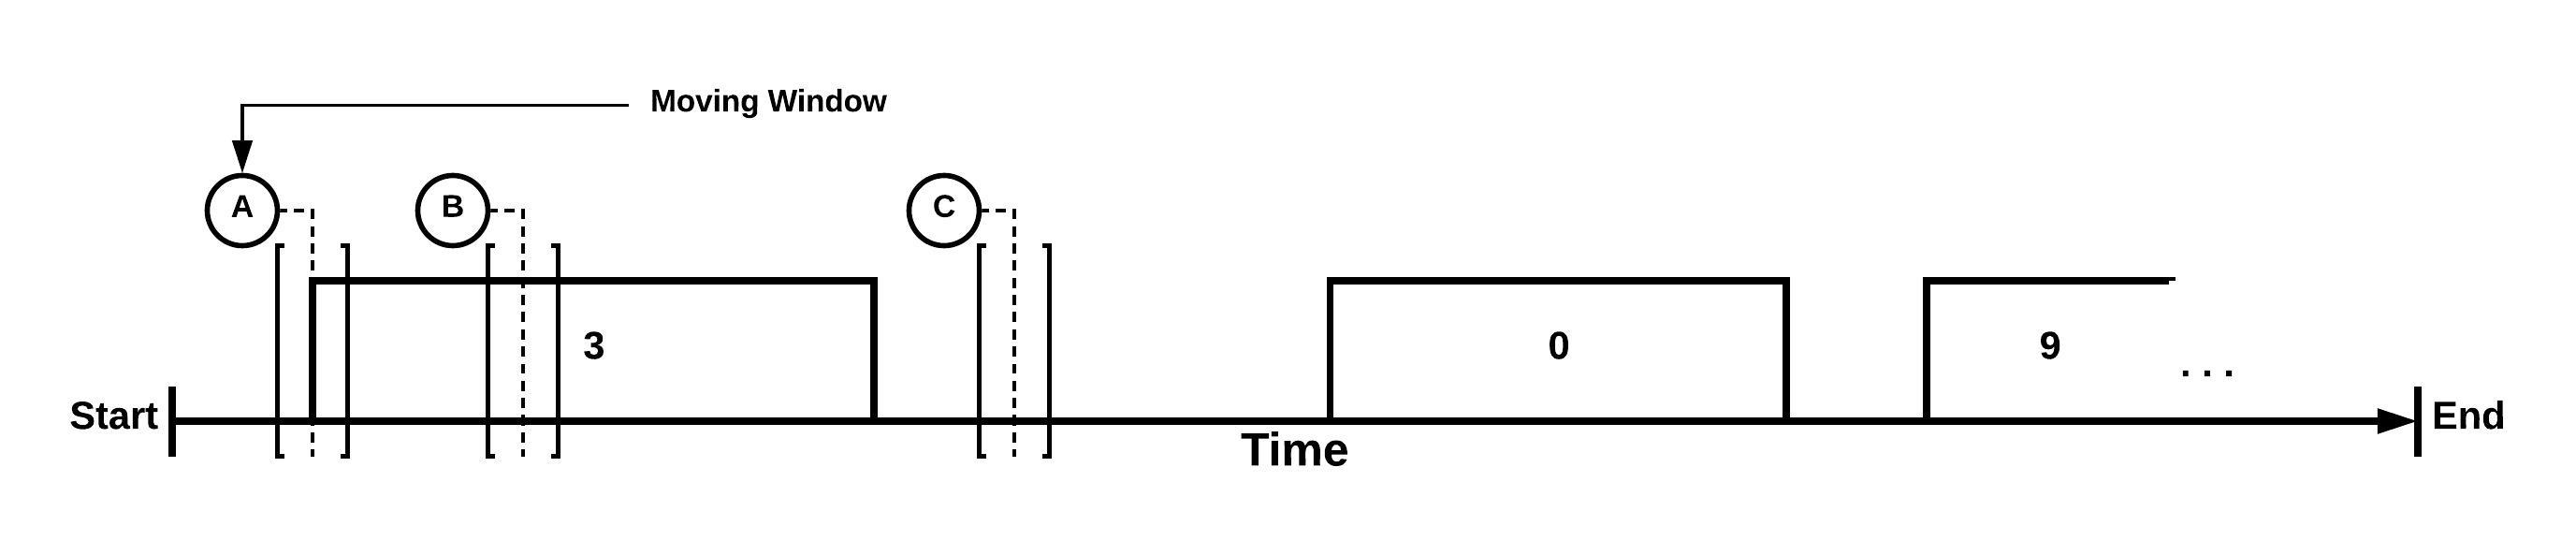
\includegraphics[width=\textwidth]{MovingDTMFDetector.JPEG}
	\end{center}
	\vspace{-1em}
	\caption{Moving window detection stages.}
	\label{WindowStages}
\end{figure}

Expressed more explicitly, Figure ~\ref{FlowDiagram} in the appendix illustrates how the process flow detects digits and avoids duplicate detection. Additionally, it shows how the DTFM function is used in the bottom left-hand box. Here we can see that each sample can be easily loaded and the phone number can be returned.


%
%%---------------------------------------------------------------------------------------------------| RESULTS
%

\section{Algorithm Results}

Inspecting the function definition under section ~\ref{DTMF}, the function takes in an argument for plotting, \textit{plt}. When this argument is set to \textit{1}, plots of each matched digit will automatically be created and saved under the Plots directory. If settings are changed and executed again then these plots will be overwritten. In addition to the \textit{plt} input, DTMF accepts a string extension (\textit{ext}) for each plot saved under its call. This enables the user to call the function under different conditions or for different samples and generate plots which are labeled specifically for that call.

Using the two inputs described above, we generated three sets of 10 plots, one plot per DTMF digit identified and one set per sample. some of these plots have been displayed on the subsequent page.

We can see that the noise becomes more prominent in the sub 600 Hz frequency range with samples 2 and 3, compare Figures ~\ref{Plots} ~\subref{S1D2}, \subref{S2D2} and \subref{S3D2}. Because \textit{TwinPeaks.m} (See ~\ref{TwinPeaks}) only checks for peaks between 600 and 2000 Hz, this noise has never become an issue. Notice in all samples that the end of the time series plot if truncated short of the end of the sound recording. Consequently, although there is sufficient noise in this range to cause a problem for samples 2 and 3, our process is unaffected by noise within this frequency range. If, on the other hand, there was noise or distortion between 600 and 2000 Hz, then our algorithm would be insufficiently robust to distinguish between noise and DTMF key presses.


%
%%---------------------------------------------------------------------------------------------------| SAMPLE PLOTS
%

\begin{figure}[h!]
	\centering
	\begin{tabular}{| c | c | c |}
		\hline
		\textbf{Sample 1}	&	\textbf{Sample 2}	&	\textbf{Sample 3} 	\\
		\hline
		\subfloat[Digit 1]{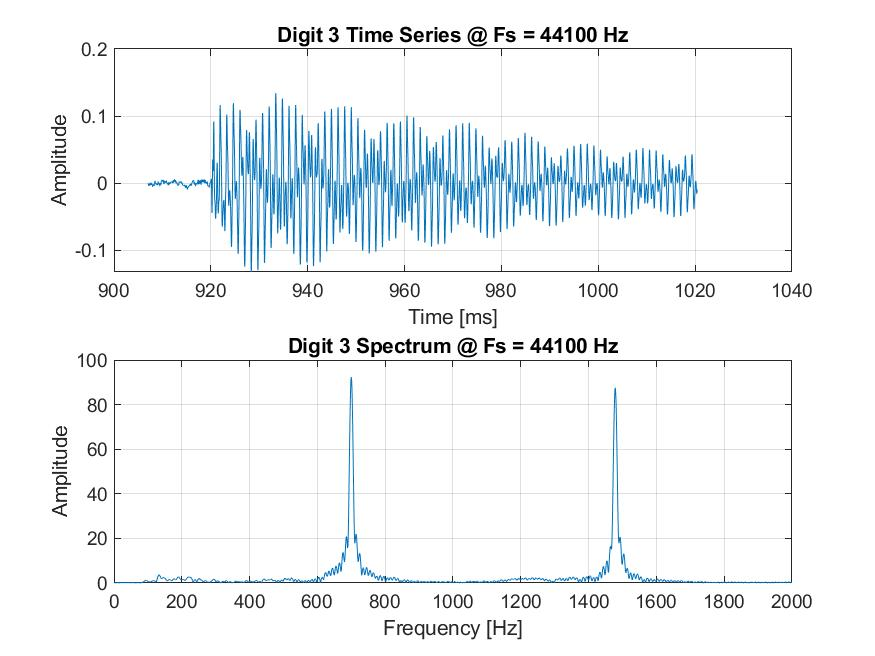
\includegraphics[width = 0.3\textwidth]{Sample1Digit1.JPEG}\label{S1D1}} &
		\subfloat[Digit 1]{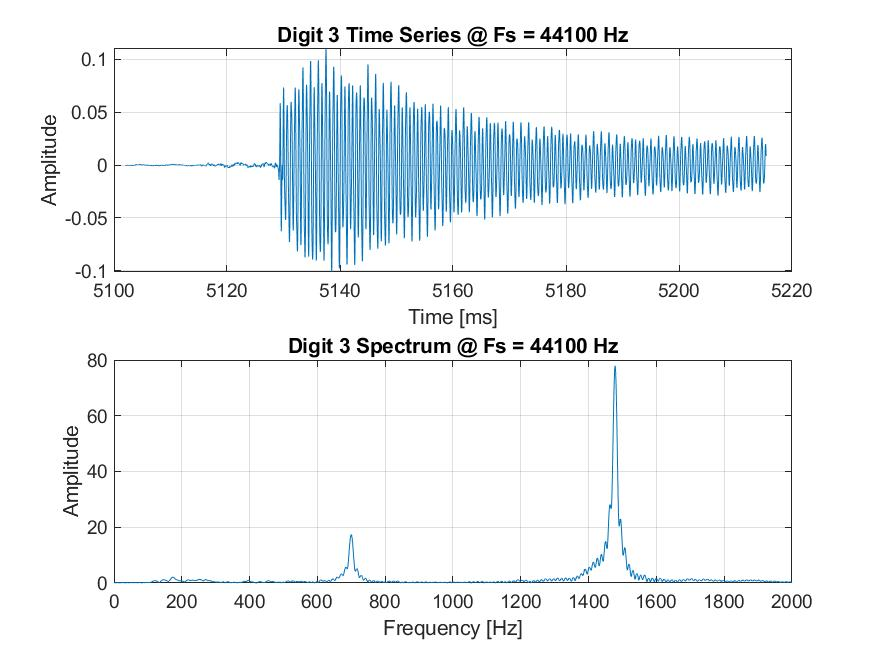
\includegraphics[width = 0.3\textwidth]{Sample2Digit1.JPEG}\label{S2D1}} &
		\subfloat[Digit 1]{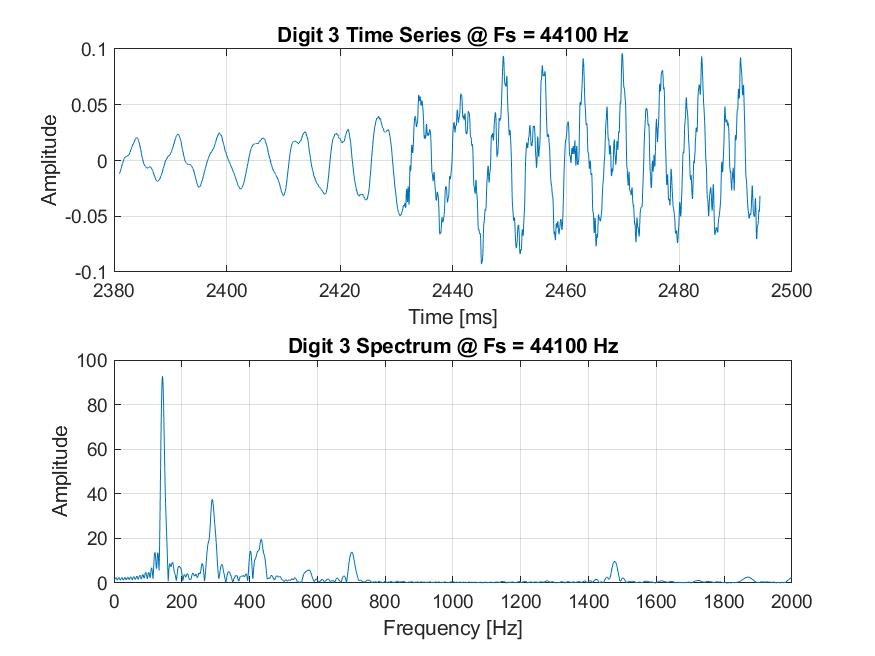
\includegraphics[width = 0.3\textwidth]{Sample3Digit1.JPEG}\label{S3D1}} \\
		\subfloat[Digit 2]{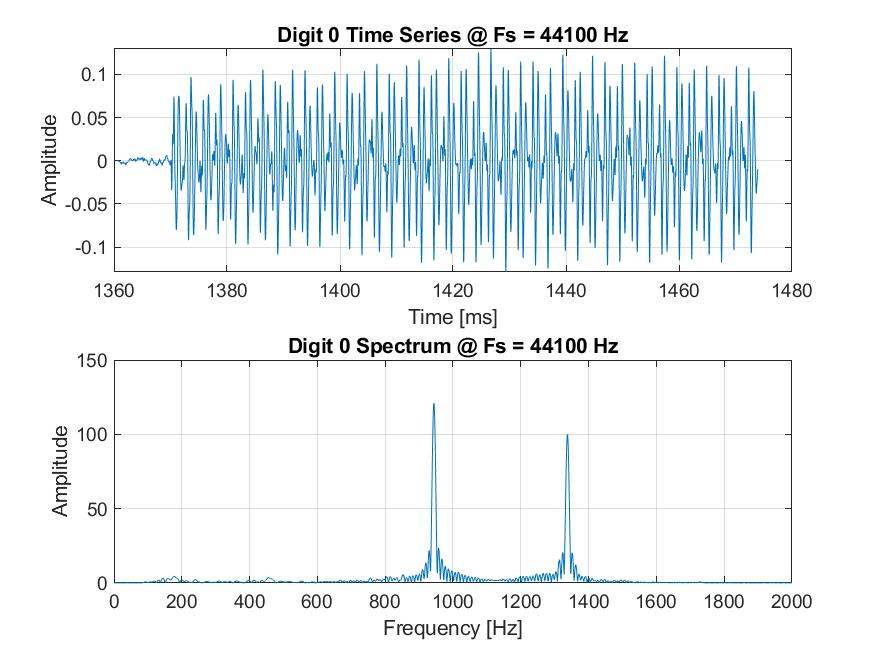
\includegraphics[width = 0.3\textwidth]{Sample1Digit2.JPEG}\label{S1D2}} &
		\subfloat[Digit 2]{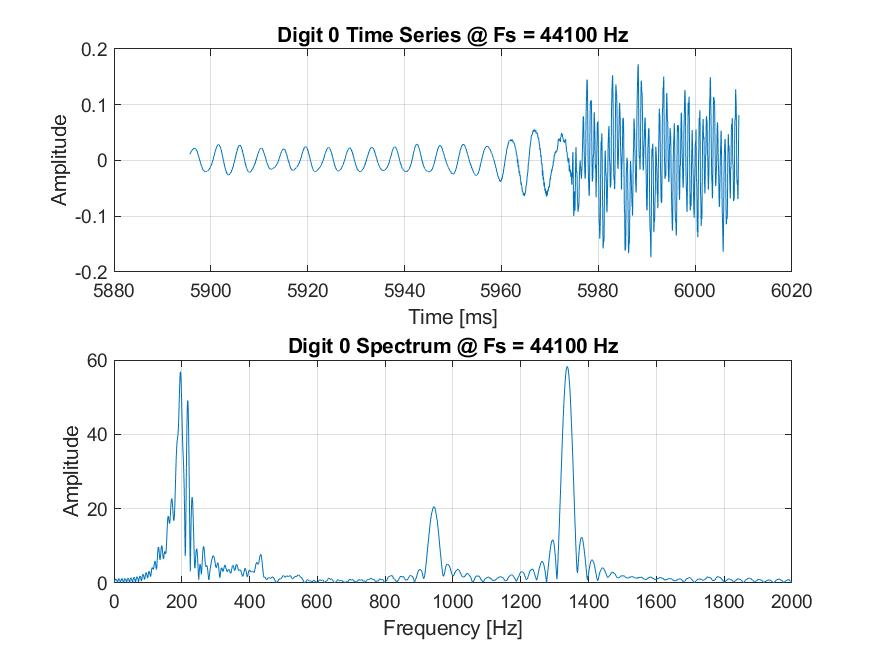
\includegraphics[width = 0.3\textwidth]{Sample2Digit2.JPEG}\label{S2D2}} &
		\subfloat[Digit 2]{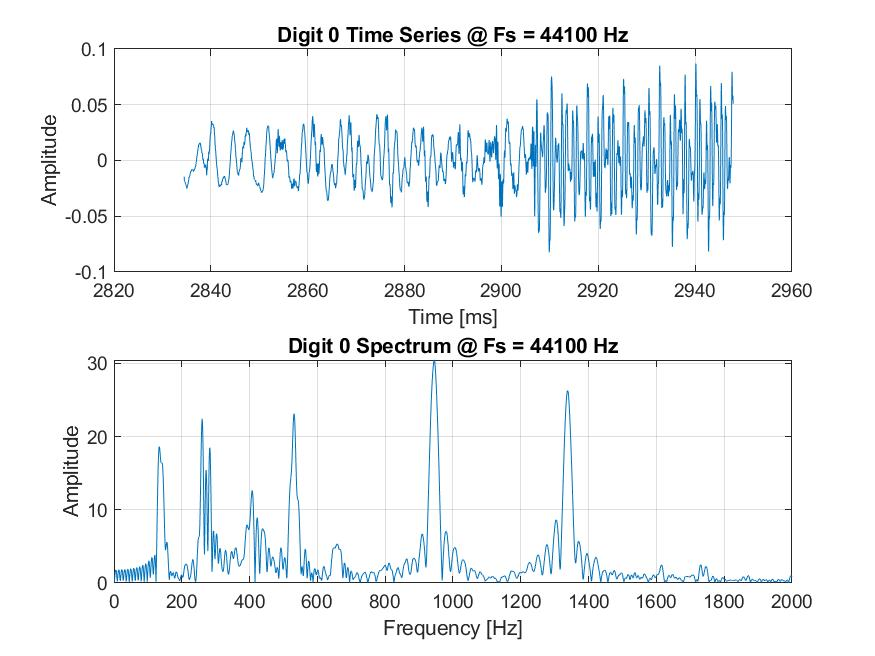
\includegraphics[width = 0.3\textwidth]{Sample3Digit2.JPEG}\label{S3D2}} \\
		\subfloat[Digit 3]{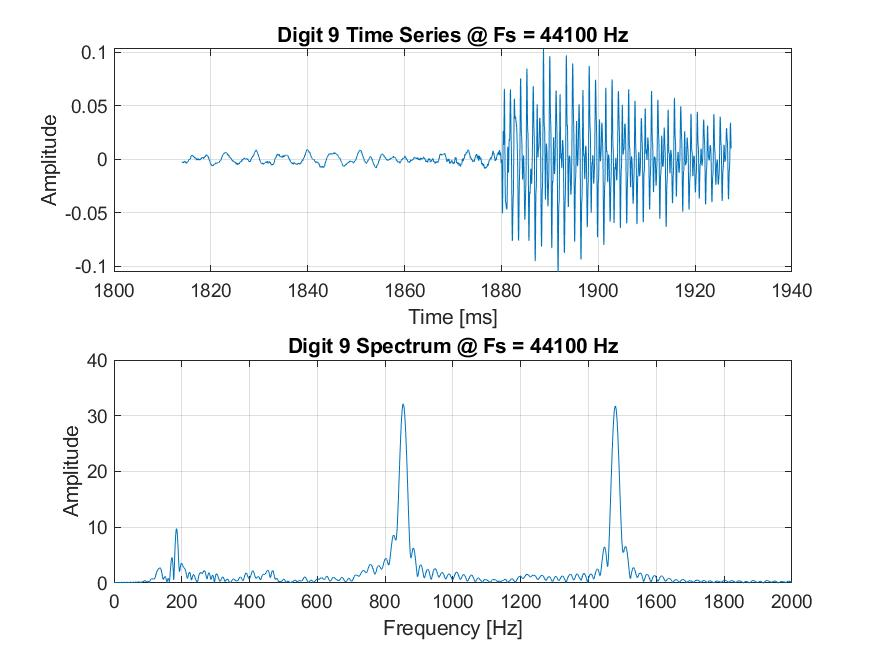
\includegraphics[width = 0.3\textwidth]{Sample1Digit3.JPEG}\label{S1D3}} &
		\subfloat[Digit 3]{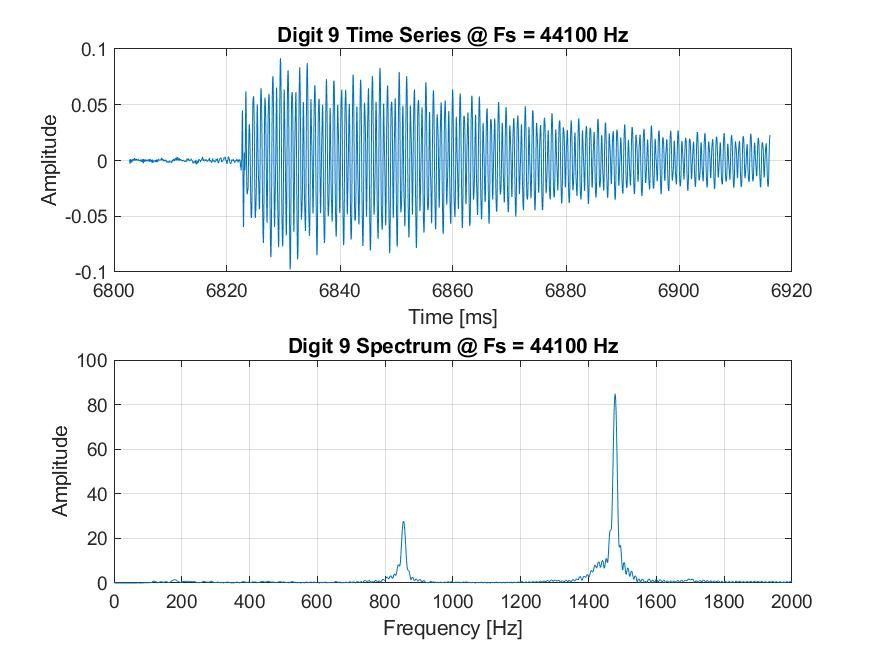
\includegraphics[width = 0.3\textwidth]{Sample2Digit3.JPEG}\label{S2D3}} &
		\subfloat[Digit 3]{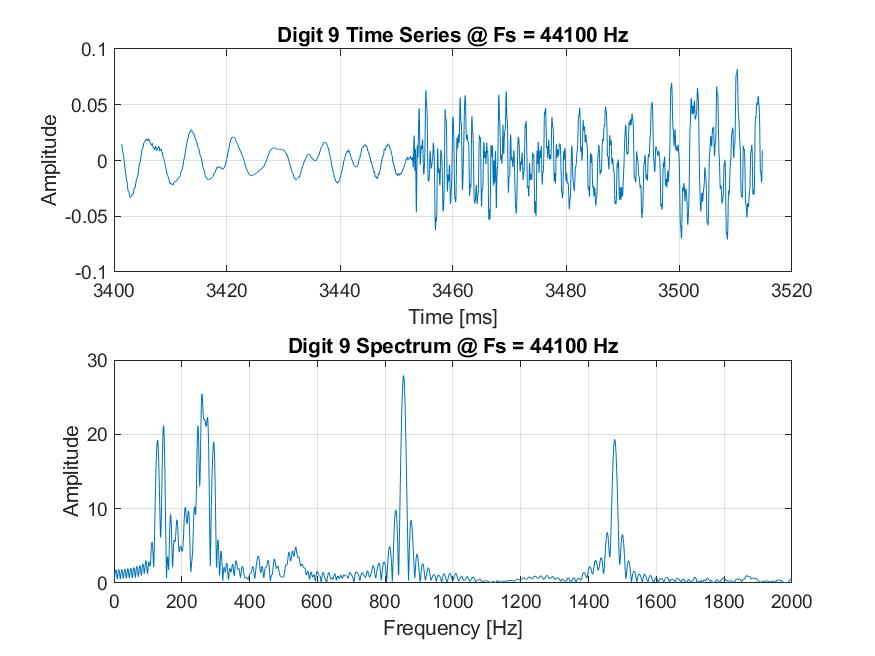
\includegraphics[width = 0.3\textwidth]{Sample3Digit3.JPEG}\label{S3D3}} \\
		\subfloat[Digit 4]{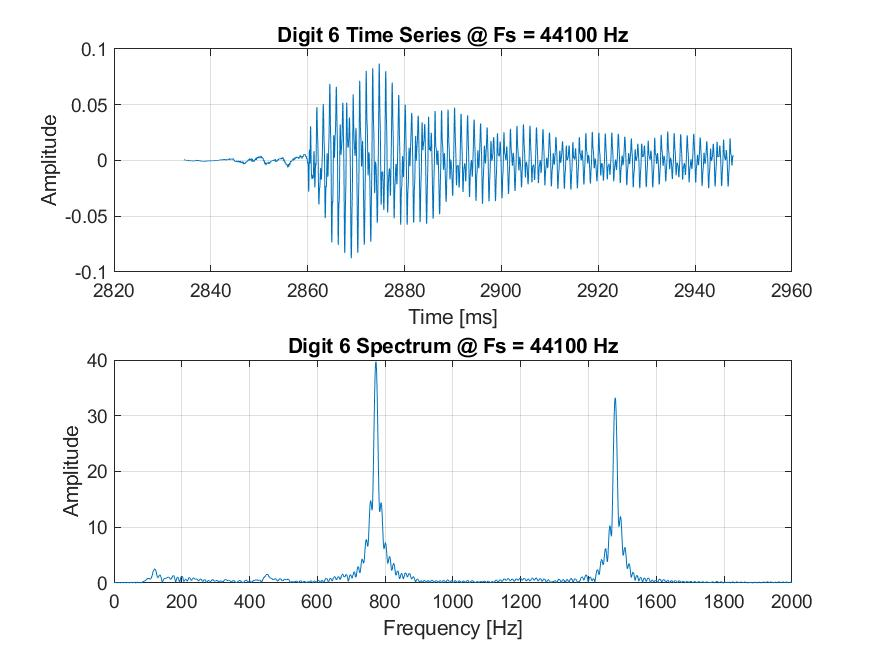
\includegraphics[width = 0.3\textwidth]{Sample1Digit4.JPEG}\label{S1D4}} &
		\subfloat[Digit 4]{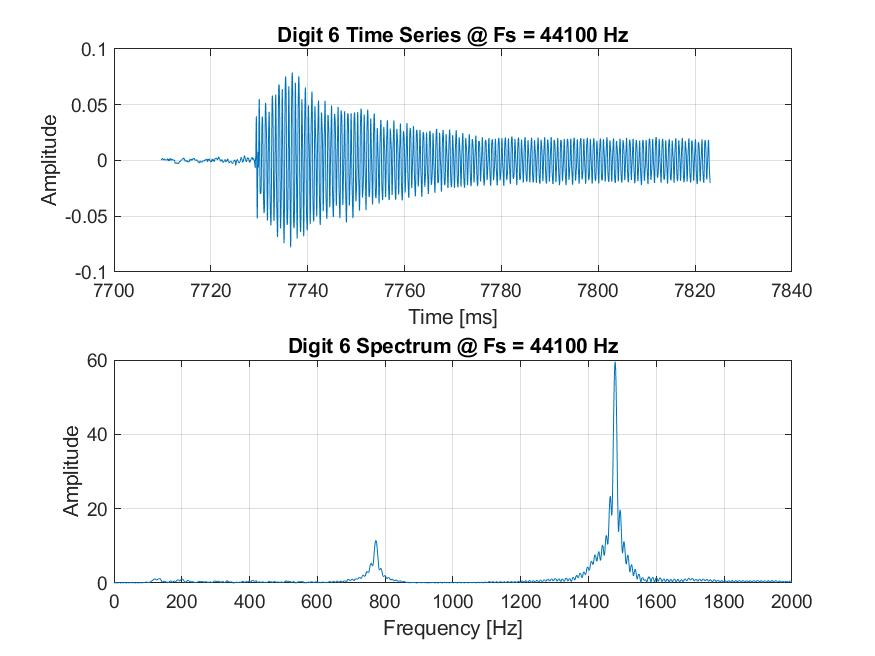
\includegraphics[width = 0.3\textwidth]{Sample2Digit4.JPEG}\label{S2D4}} &
		\subfloat[Digit 4]{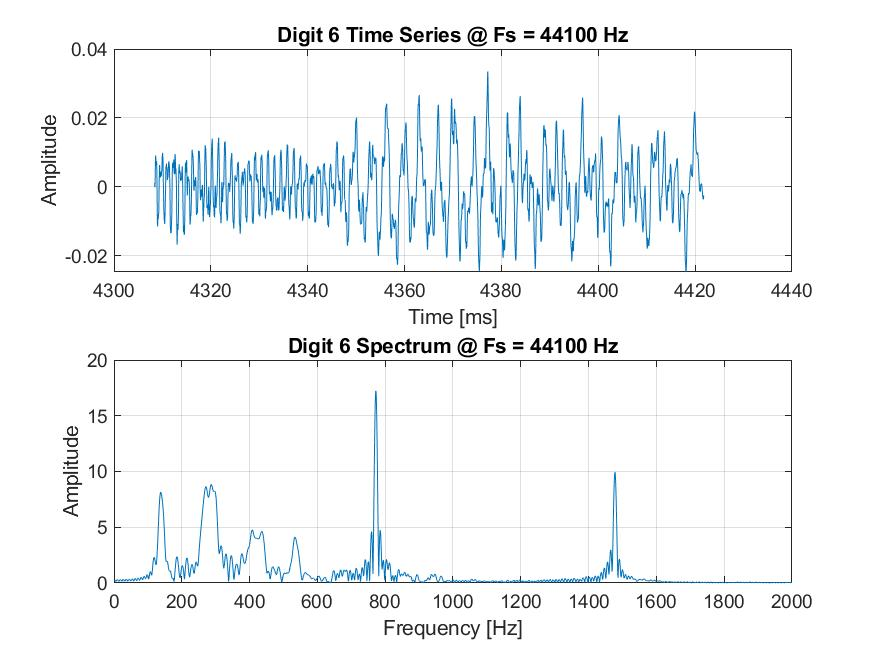
\includegraphics[width = 0.3\textwidth]{Sample3Digit4.JPEG}\label{S3D4}} \\
		\hline
	\end{tabular}
	\vspace{0.2cm}
	\caption{First four digit readings per sample.}
	\label{Plots}
\end{figure}


%
%%---------------------------------------------------------------------------------------------------| RESULTS CONT.
%
\vspace{1cm}
As we mentioned earlier, our solution can scan, plot, and return DTMF key presses quicker than previous solutions. Using MATLABs \textit{tic toc} commands we timed the performance of our DTMF calls. After each iteration it became faster due to MATLABs dynamic memory allocation but it consistently performed key detection in under half a second, see the appendix for Figure ~\ref{Speed}.


%
%%---------------------------------------------------------------------------------------------------| APPENDIX
%

\clearpage
\section{Appendix}

\begin{figure}[h!]
	\begin{center}
		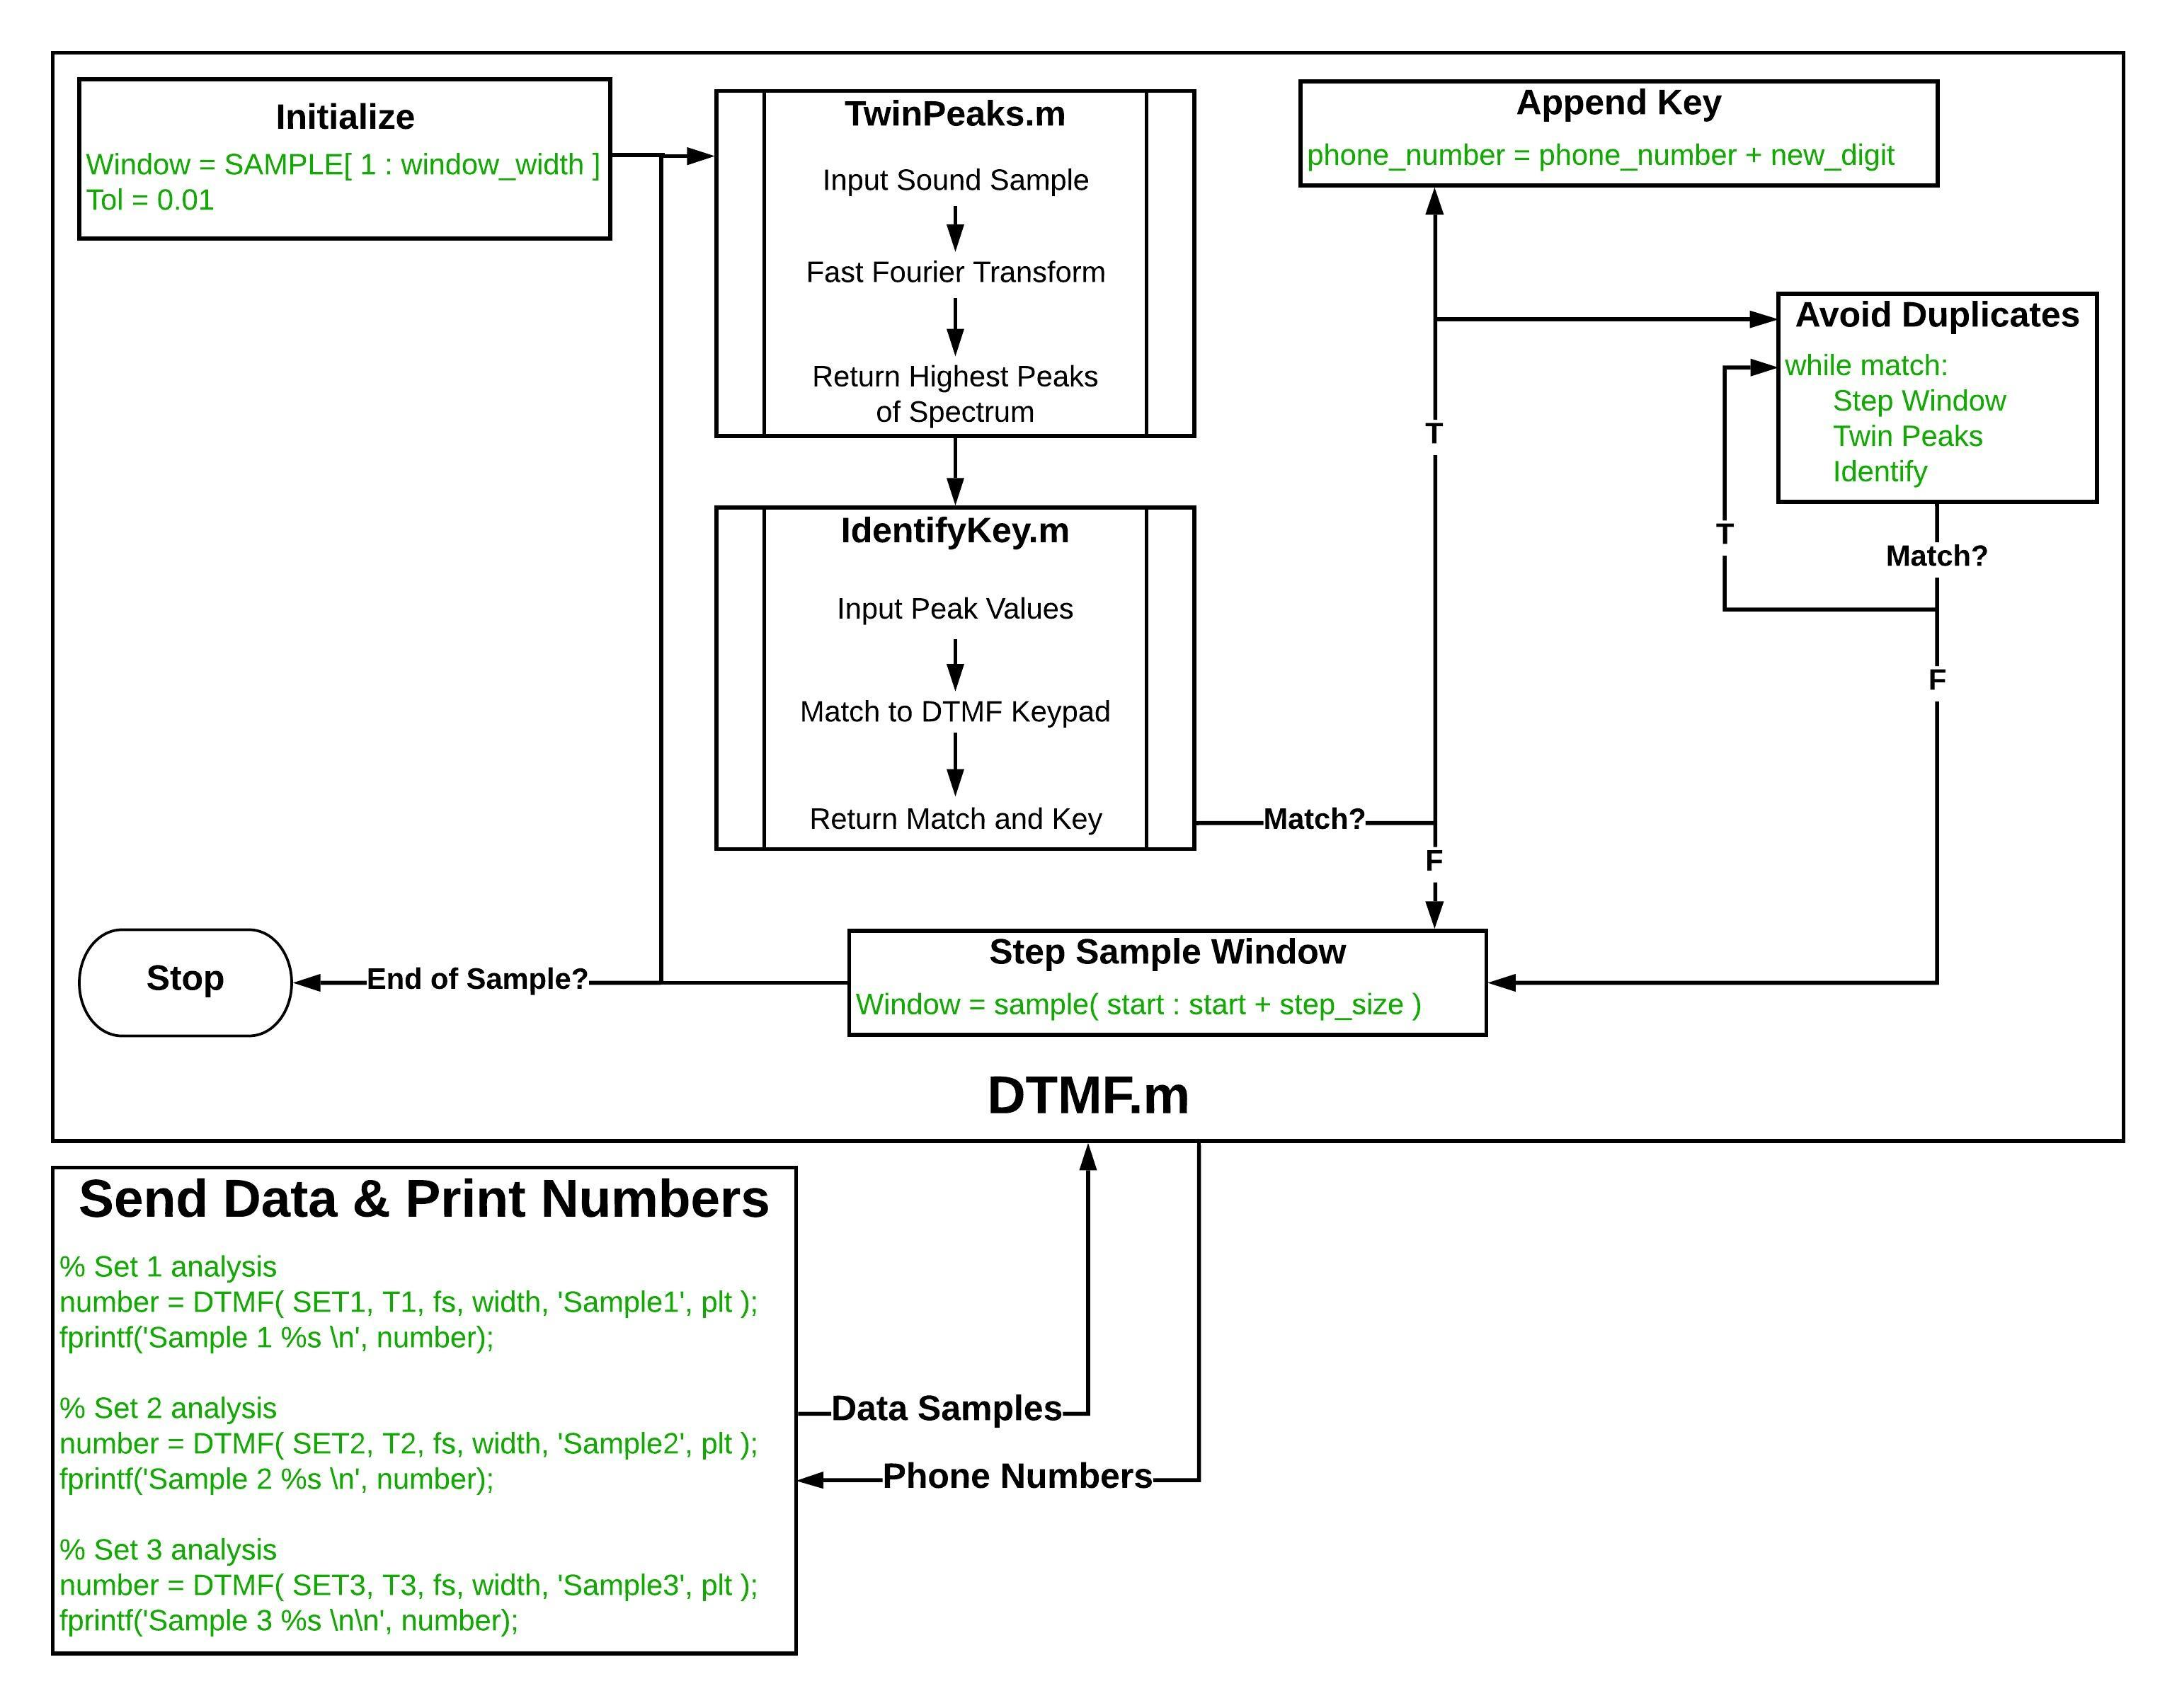
\includegraphics[width=\textwidth]{FlowDiagram.JPEG}
	\end{center}
	\vspace{-1em}
	\caption{Broad program ecosystem.}
	\label{FlowDiagram}
\end{figure}

\begin{figure}[h!]
	\begin{center}
		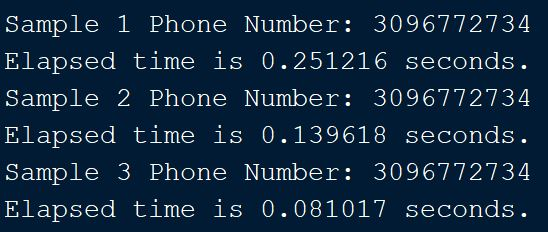
\includegraphics[width=0.5\textwidth]{Speed.JPEG}
	\end{center}
	\vspace{-1em}
	\caption{DTMF speed test.}
	\label{Speed}
\end{figure}



\end{document}

